\documentclass{beamer}

\usepackage{amsmath,amssymb,amsfonts}
\usepackage{amsthm}
\usepackage{mathtools}  % For \DeclarePairedDelimiter
\usepackage{graphicx}
\usepackage{hyperref}
\usepackage{algorithm}
\usepackage{algpseudocodex}
\usepackage{siunitx}
\usepackage{booktabs}
\usepackage{caption}
\usepackage{subcaption}
\usepackage{cleveref}
\usepackage{physics}
\usepackage{bm}

% Custom commands from the paper
\newcommand{\R}{\mathbb{R}}
\newcommand{\N}{\mathbb{N}}
\newcommand{\E}{\mathbb{E}}
\let\P\relax
\newcommand{\P}[1]{\mathbb{P}\left[#1\right]}
\newcommand{\normal}{\mathcal{N}}
\newcommand{\diag}[1]{\mathrm{diag}(#1)}
\DeclareMathOperator*{\minimize}{minimize}

% Set path for figures
\graphicspath{{../figures/}}

% Beamer theme
\usetheme[progressbar=frametitle]{metropolis}

\title{Square Root QR Covariance Steering}
\subtitle{A Novel Approach for Chance-Constrained Covariance Steering}
\author{Naoya Kumagai, Kenshiro Oguri}
\institute{School of Aeronautics and Astronautics, Purdue University}
\date{\today}

\begin{document}

% Title slide
\frame{\titlepage}

\section{Introduction}

\begin{frame}{Covariance Steering (CS)}
\begin{itemize}
    \item Control framework that explicitly addresses uncertainty
    \item Steers both \textbf{mean} and \textbf{covariance} to desired values
    \item Yields optimal feedforward + feedback control policies
    \item Applications: spacecraft rendezvous, safe navigation, etc.
\end{itemize}

\vspace{0.5cm}
\textbf{Challenge:} Numerical issues when variance is small compared to mean
\end{frame}

\begin{frame}{Motivation: Numerical Issues}
\begin{columns}
\begin{column}{0.5\textwidth}
\textbf{Existing Methods:}
\begin{itemize}
    \item Block-matrix approaches: poor scalability
    \item Full-covariance methods: numerical instability
    \item Small variance $\rightarrow$ squared units $\rightarrow$ ill-scaling
\end{itemize}
\end{column}
\begin{column}{0.5\textwidth}
\textbf{Square Root Filtering:}
\begin{itemize}
    \item Used in Apollo Guidance Computer
    \item ``Half as many bits'' of precision needed
    \item More numerically stable
\end{itemize}
\end{column}
\end{columns}

\vspace{0.5cm}
\textbf{Our Approach:} Use Cholesky factor (square root) of covariance matrix as optimization variable
\end{frame}

\begin{frame}{Contributions}
\begin{enumerate}
    \item \textbf{Square root formulation} using QR decomposition
    \begin{itemize}
        \item Better numerical reliability
        \item Flexible cost formulation
    \end{itemize}
    
    \item \textbf{Sequential Convex Programming (SCP)} solution
    \begin{itemize}
        \item Globally optimal for unconstrained quadratic case
        \item Locally optimal in general
    \end{itemize}
    
    \item \textbf{Computational advantages}
    \begin{itemize}
        \item Better scalability than block-matrix methods
        \item Memoryless feedback control
        \item Superior numerical stability
    \end{itemize}
\end{enumerate}
\end{frame}

\section{Problem Formulation}

\begin{frame}{Problem Statement}
\begin{block}{Discrete-Time Covariance Steering}
\begin{align*}
&\minimize_{\boldsymbol{v}, \boldsymbol{K}} \quad J = \sum_{k=0}^{N-1} J_k (x_k, u_k) \\
&\text{subject to} \\
& x_{k+1} = A_k x_k + B_k u_k + G_k w_k \\
& u_k = v_k + K_k (x_k - \E{x_k}) \\
& x_0 \sim \normal(\mu_{\mathrm{init}}, P_{\mathrm{init}}) \\
& \mu_{\mathrm{fin}} = \E{x_N} \\
& P_{\mathrm{fin}} \succeq \E{(x_N - \E{x_N})(x_N - \E{x_N})^\top} \\
& \mathbb{P}(x_k \in \mathcal{X}) \geq 1 - \epsilon_x \\
& \mathbb{P}(u_k \in \mathcal{U}) \geq 1 - \epsilon_u
\end{align*}
\end{block}
\end{frame}

\begin{frame}{Covariance Propagation}
\begin{block}{Standard Form}
\[
P_{k+1} = (A_k + B_k K_k) P_k (A_k + B_k K_k)^T + G_k G_k^\top
\]
\end{block}

\begin{block}{Square Root Form (Our Approach)}
\[
S_{k+1} = \mathrm{qr}(X_{k+1}^\top)^\top, \quad X_{k+1} = \begin{bmatrix} (A_k + B_k K_k) S_k & G_k \end{bmatrix}
\]
where $S_k = P_k^{1/2}$ is the Cholesky factor
\end{block}

\vspace{0.3cm}
\textbf{Key Insight:} QR decomposition ensures $S_{k+1} \in \mathbb{L}_+^n$ (lower triangular with positive diagonal)
\end{frame}

\begin{frame}{Change of Variables}
To handle bilinear term $K_k S_k$, we define:
\[
L_k = K_k S_k \quad \Rightarrow \quad K_k = L_k S_k^{-1}
\]

Then the square root propagation becomes:
\[
S_{k+1} = \mathrm{qr}(X_{k+1}^\top)^\top, \quad X_{k+1} = \begin{bmatrix} A_k S_k + B_k L_k & G_k \end{bmatrix}
\]

\vspace{0.3cm}
\textbf{Nonconvexity:} The QR operation is nonlinear, requiring iterative solution
\end{frame}

\section{Method}

\begin{frame}{QR Decomposition Derivative}
For optimization, we need the derivative of QR decomposition:

\[
\mathrm{d} R = Q^\top (\mathrm{d} M) - \mathrm{tril}(Q^\top (\mathrm{d} M) R^{-1}) R
\]

Linearization around reference $\bar{M} = \bar{Q} \bar{R}$:
\[
\mathrm{qr}(M) \approx \bar{R} + \mathrm{d} R(M - \bar{M}, \bar{Q}, \bar{R})
\]

This enables sequential convex programming!
\end{frame}

\begin{frame}{Sequential Convex Programming (SCP)}
\begin{block}{Algorithm: SCvx*}
At each iteration:
\begin{enumerate}
    \item Linearize square root dynamics using QR derivative
    \item Solve convex subproblem with trust region
    \item Update reference trajectory if step accepted
    \item Update Lagrange multipliers and penalty weights
\end{enumerate}
\end{block}

\vspace{0.3cm}
\textbf{Convergence:} Guaranteed to local optimum (global for unconstrained quadratic case)
\end{frame}

\begin{frame}{Convex Subproblem}
\begin{block}{Linearized Dynamics}
\[
\mathrm{vectril} \left\{ S_{k+1} - \mathrm{qr}(\bar{X}_{k+1}^\top)^\top - \mathrm{d} R(X_{k+1}^\top - \bar{X}_{k+1}^\top, \bar{Q}_{k+1}, \bar{R}_{k+1})^\top \right\} = \boldsymbol{\xi}_k
\]
\end{block}

\begin{block}{Trust Region}
\[
\lVert\mathrm{vec}(D_X(X_k - \bar{X}_k))\rVert_\infty \leq r
\]
\end{block}

\begin{block}{Augmented Lagrangian}
\[
\mathcal{L} = J(\boldsymbol{z}) + P(\boldsymbol{\xi}; w, \boldsymbol{\lambda})
\]
\end{block}
\end{frame}

\section{Theoretical Results}

\begin{frame}{Optimality Guarantees}
\begin{theorem}[Local Optimality]
The SCP algorithm converges to a locally optimal solution, and this local optimality is invariant to whether we use full covariance or square root representation.
\end{theorem}

\begin{theorem}[Global Optimality]
When chance constraints are absent and the objective is quadratic, the solution is \textbf{globally optimal}.
\end{theorem}

\vspace{0.3cm}
\textbf{Key:} Cholesky map is a diffeomorphism, preserving optimality structure
\end{frame}

\section{Numerical Examples}

\begin{frame}{Scalability Comparison}
\begin{columns}
\begin{column}{0.5\textwidth}
\begin{figure}
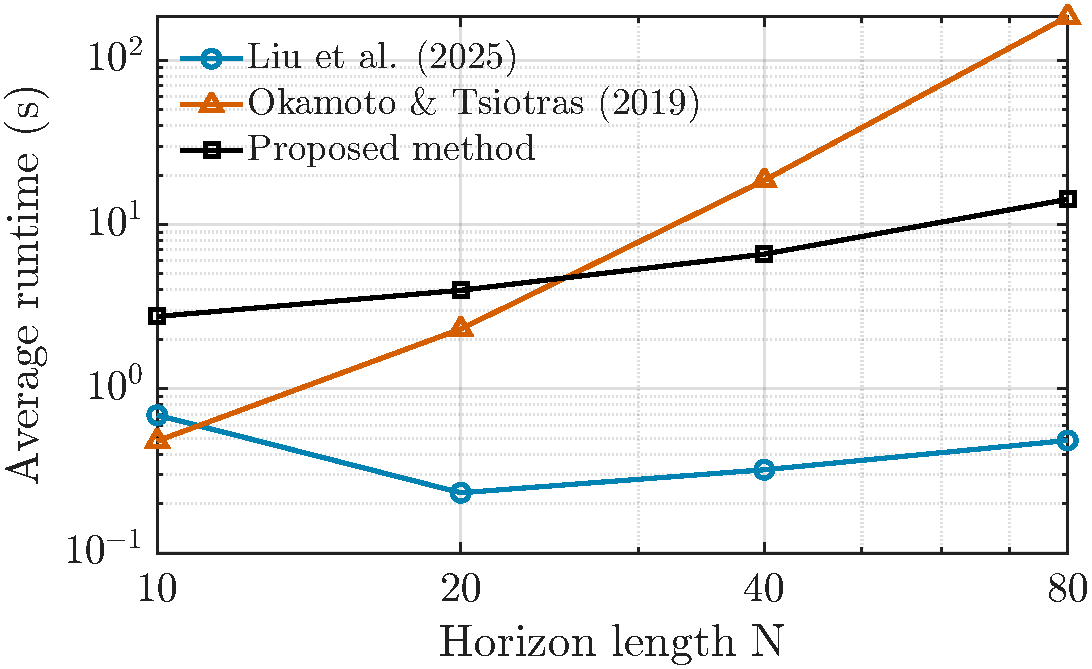
\includegraphics[width=\textwidth]{horizon_size_scalability.pdf}
\caption{Solution time vs horizon length}
\end{figure}
\end{column}
\begin{column}{0.5\textwidth}
\begin{figure}
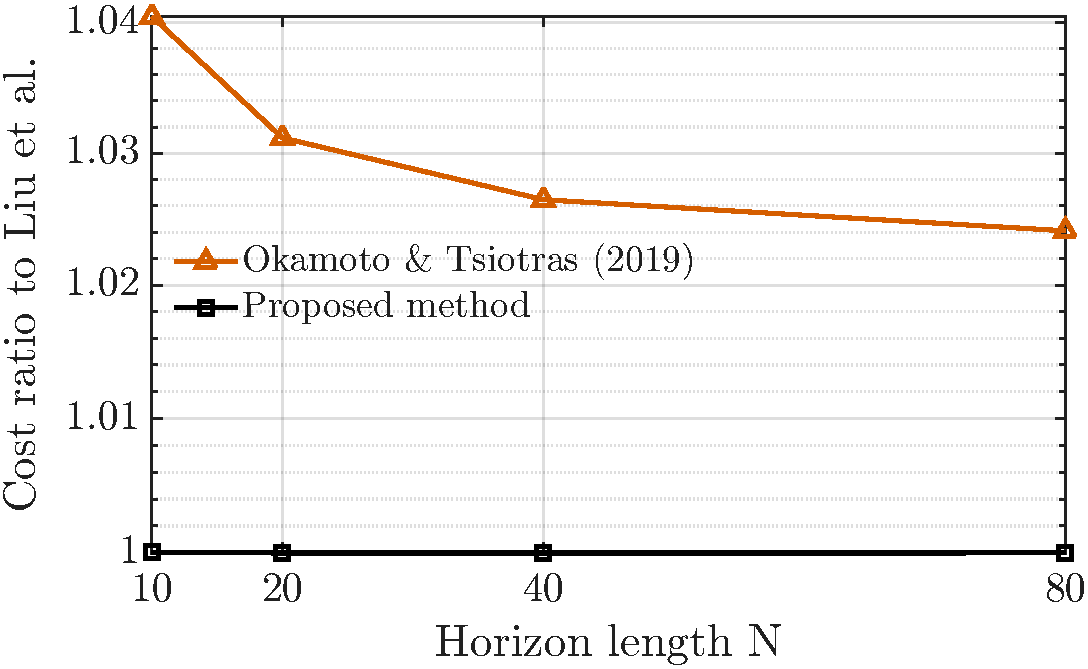
\includegraphics[width=\textwidth]{horizon_size_cost_comparision.pdf}
\caption{Cost comparison}
\end{figure}
\end{column}
\end{columns}

\vspace{0.3cm}
\textbf{Results:}
\begin{itemize}
    \item Better scalability than block-matrix methods
    \item Achieves optimality (matches Liu et al.)
    \item Memoryless feedback control
\end{itemize}
\end{frame}

\begin{frame}{Numerical Reliability: Spacecraft Rendezvous}
\begin{columns}
\begin{column}{0.5\textwidth}
\begin{figure}
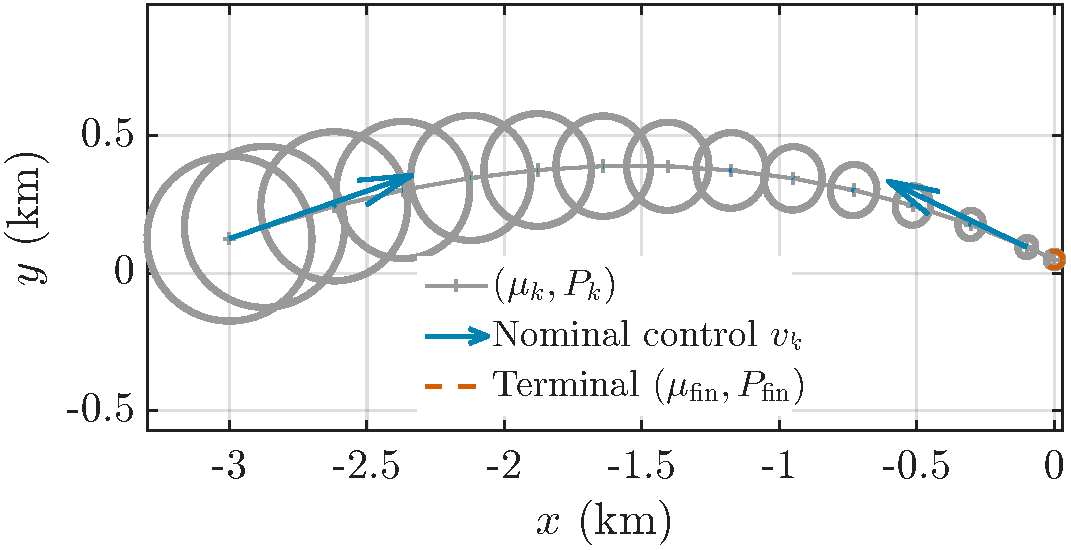
\includegraphics[width=\textwidth]{example_cwh_trajectory.pdf}
\caption{Trajectory with 3$\sigma$ ellipses}
\end{figure}
\end{column}
\begin{column}{0.5\textwidth}
\textbf{Problem:}
\begin{itemize}
    \item Small position uncertainty (100m)
    \item Large mean position (3km)
    \item QoN objective function
\end{itemize}

\vspace{0.3cm}
\textbf{Results:}
\begin{itemize}
    \item Proposed method: 42 iterations, 5.0s
    \item Full-covariance: \textbf{FAILED} (numerical issues)
\end{itemize}
\end{column}
\end{columns}
\end{frame}

\begin{frame}{Covariance Propagation Accuracy}
\begin{figure}
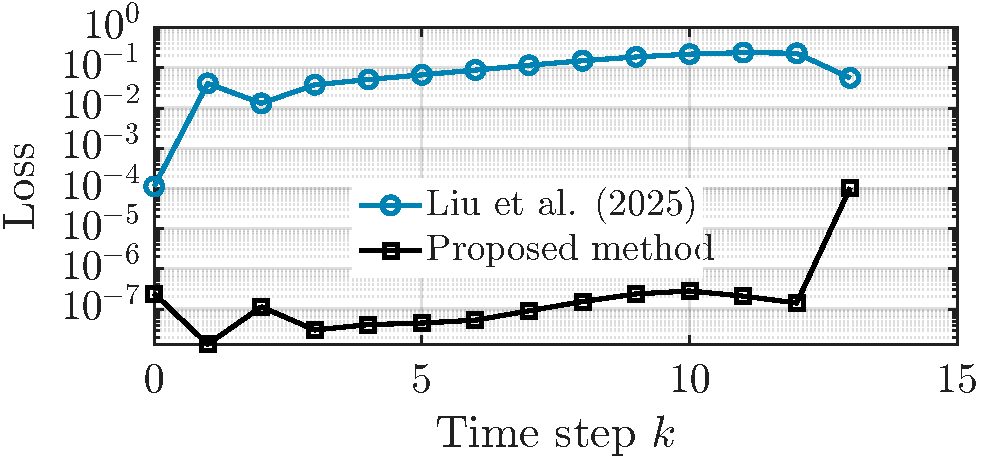
\includegraphics[width=0.7\textwidth]{example_cwh_covariance_propagation_loss.pdf}
\caption{Covariance propagation loss}
\end{figure}

\vspace{0.3cm}
\textbf{Key Finding:} Square root method maintains accurate covariance propagation even with tight tolerances
\end{frame}

\section{Conclusions}

\begin{frame}{Summary}
\begin{block}{Benefits of Square Root Approach}
\begin{itemize}
    \item \textbf{Numerical reliability} for small variance problems
    \item \textbf{Flexible cost formulation} (beyond quadratic)
    \item \textbf{Good scalability} with horizon length
    \item \textbf{Memoryless feedback} control law
    \item \textbf{Global optimality} for unconstrained quadratic case
\end{itemize}
\end{block}

\vspace{0.5cm}
\textbf{Trade-off:} Iterative SCP approach vs. single-shot convex optimization
\begin{itemize}
    \item But: Offline computation, online is cheap
    \item Flexibility and stability often worth the cost
\end{itemize}
\end{frame}

\begin{frame}{Future Work}
\begin{itemize}
    \item Extension to continuous-time systems
    \item Non-Gaussian uncertainty
    \item Real-time applications with warm-starting
    \item Integration with learning-based methods
\end{itemize}
\end{frame}

\begin{frame}[plain]
    \centering
    \vspace{2cm}
    
    \Huge Thank You!
    
    \vspace{1cm}
    
    \Large Questions?
    
    \vspace{1.5cm}
    
    \normalsize
    Code: \texttt{https://github.com/naoya-kumagai/}\\
    \texttt{sqrt\_covariance\_steering/}
\end{frame}

\end{document}

